\documentclass{beamer}
\usepackage[utf8]{inputenc}
\usetheme{Madrid}
\usecolortheme{beaver}
\usepackage{graphicx}

\usepackage[export]{adjustbox}


\title{Constraining the Astrophysical R-Process}
\author[Kieran Porter]{Kieran Porter \newline{\tiny Supervisor: Dan Watts}}


\date{January 2017}

\begin{document}

\maketitle

%----------------- This Project -------------------------------------------------------

\begin{frame}{This Project}
\begin{itemize}
    \item Analyse data from proton knockout experiments using $^{208}Pb$ and $^{12}C$ targets.
    \item Determine masses of residual exotic nuclei.
    \item Study how number of events changes with number of protons knocked out.
    \item (Possibly deduce energy level structures.)
    \item Provide experimental data to constrain path of the r-process and test
    theoretical models.
\end{itemize}

\end{frame}


%------------------ Stellar Nucleosynthesis ---------------------------------------

\begin{frame}{Stellar Nucleosynthesis}
%\begin{itemize}
  %  \item Fusion processes up to $^{56}Fe$, $Z=26$.
 %   \item Coulomb barrier quickly becomes too great for charged particle induced reactions at $Z>26$.
%\end{itemize}
    
    
        \centering
        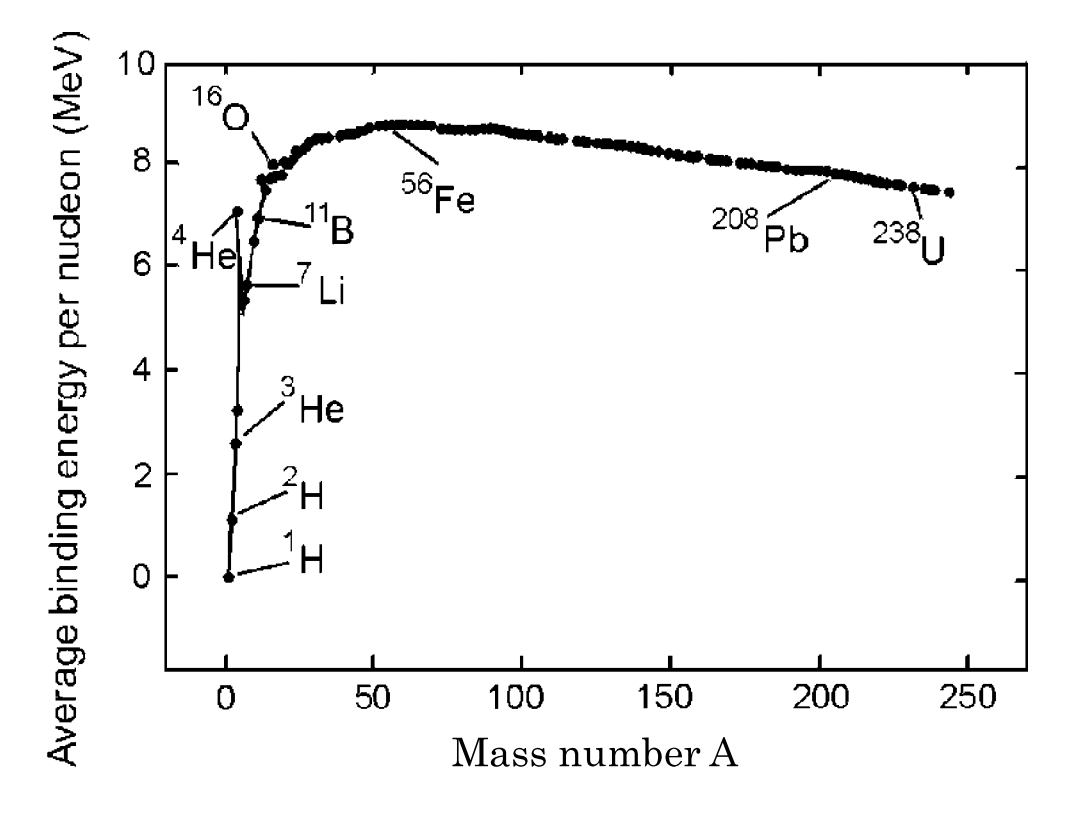
\includegraphics[height = 7cm]{BindingEnergy}
        \\{\tiny Kamal, A. "Nuclear Physics", Berlin : Springer (2014).}
       
    
\end{frame}

%------------------ R-Process 1 ------------------------------------------------------

\begin{frame}{R-Process}

\begin{itemize}
    \item Very high flux of neutrons available.
    \item Neutron capture rate``rapid" relative to $\beta$-decay rate.
\end{itemize}

        \centering
        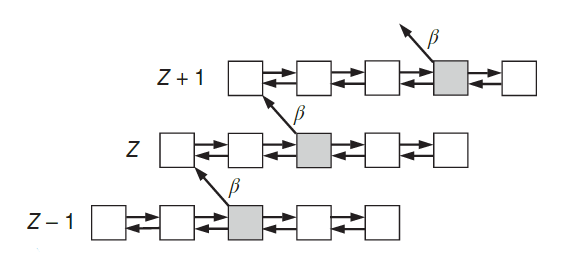
\includegraphics[height=6cm]{isotopicChain2}
        \\{\tiny Iliadis, C. ``Nuclear Physics of Stars", Weinheim, Germany : Springer (2015).}

\end{frame}

%----------------- R-Process 2 -------------------------------------------------------
\begin{frame}{Shell Influences}
    \begin{itemize}
        \item Pile up of abundance along shell closures.
    \end{itemize}
    
       \centering
        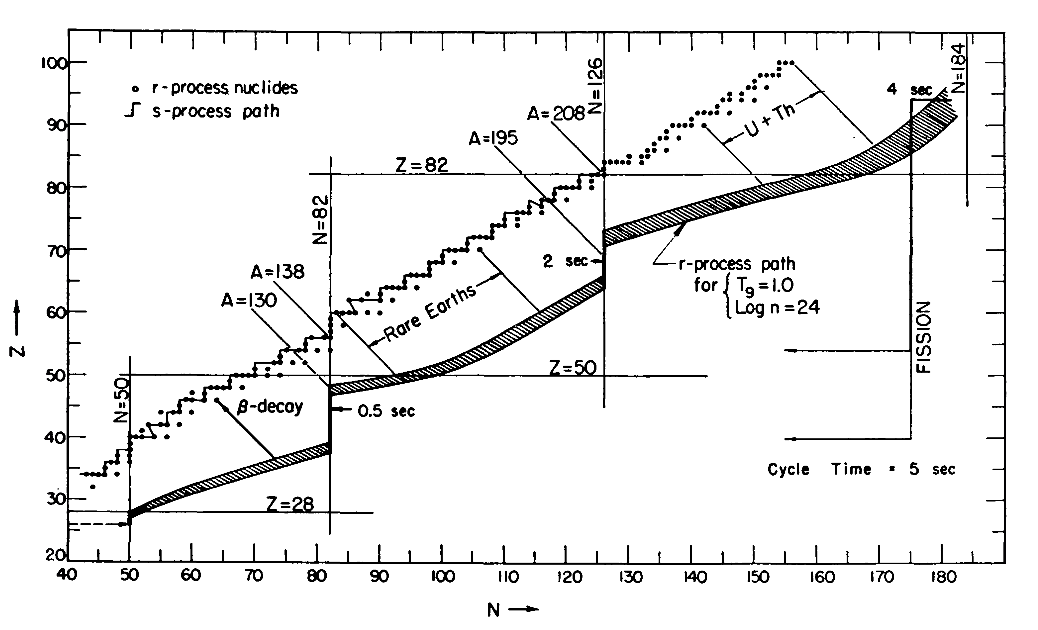
\includegraphics[height = 5.5cm]{RProcessPath}
       \\{\tiny Seeger, P.A., Fowler, W.A., Clayton, D.D. \textit{AstroPhys. J. Suppl} \textbf{11} (1965).}
       
       
\end{frame}

%------------------ R-Process Problems -------------------

\begin{frame}{The Problem}

\begin{itemize}
    \item R-Process path wonders very far from stability.
    \item Theoretical models do not predict observed abundance correctly.
    \item Majority of nuclei never observed.
    \item Very little experimental data on exotic nuclei.
    \item Does shell structure even persist for exotic nuclei?
\end{itemize}

\centering
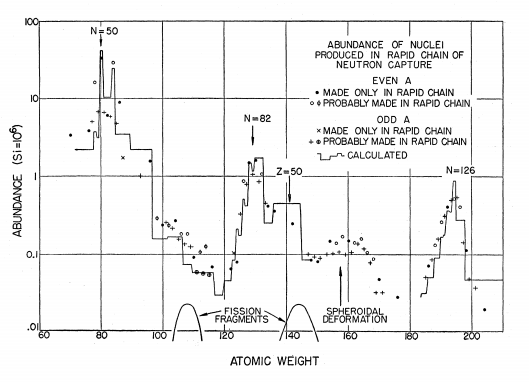
\includegraphics[height =5cm]{Abundances}
     \\{\tiny Burbidge, E.M., Burbidge, G.R., Fowler, W.A., Hoyle, F. \textit{Rev. Mod. Phys.} \textbf{29} (1957).}

\end{frame}


%---------------- Proton Knockout at MAMI ---------------------------------------------

\begin{frame}{Proton Knockout At MAMI}
\begin{itemize}
    \item Use electron beam to produce photons by Bremstrahlung and direct onto target.
    \item Photons knockout nucleons via several processes (eg. $\pi^{0}$ production).
    \item Use Crystal Ball detector and Particle Identification Detector (PID) to measure knockout proton energies.
    \item Reconstruct missing mass of nuclei.
\end{itemize}

    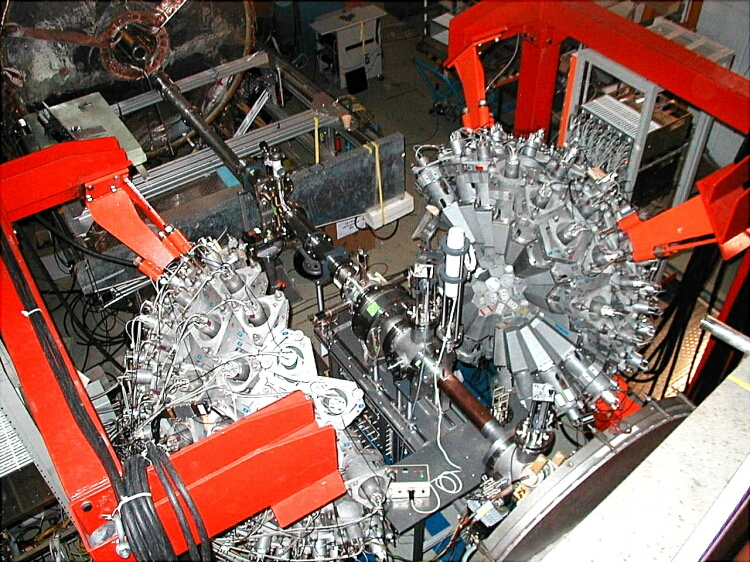
\includegraphics[height = 4cm, right]{openCB}

\end{frame}

%-------------- Data Calibration -------------------------------------------------------

\begin{frame}{Energy Calibration}

\begin{itemize}
    \item Energy lost escaping target, travelling through PID etc.
    \item "Interesting" signal lost in noise.
    \item Use Geant4 Monte-Carlo simulation to model energy losses and calculate corrections.
\end{itemize}

    \centering
    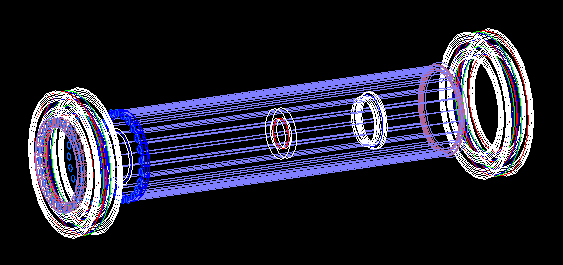
\includegraphics[height= 5cm]{AllIn}

\end{frame}

%---------------- Initial Results -----------------------
\begin{frame}{Initial Results}

\begin{itemize}
    \item Fresh from GoAT, courtesy of Prof. Dan Watts.
    \item Possible first measurement of $^{204}Pb$ mass!
\end{itemize}
\centering
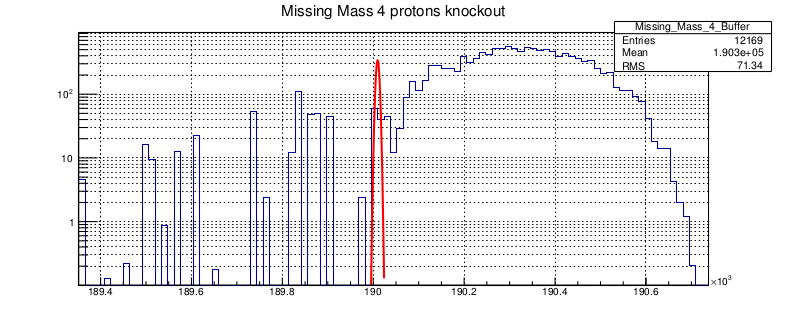
\includegraphics[width=12cm]{DanResult}
    
\end{frame}

%-------------- Conclusions/Future Work ------------------------
\begin{frame}{Conclusions and Future Work}
\begin{itemize}
    \item Will hopefully measure masses of exotic nuclei south of $^{208}Pb$!
    \item Equivalent data for $^{12}C$ ready to go.
    \item Provide constraints for r-process path.
    \item Possible implications for neutron stars ($^{7}H$).
    \item Possible implications for neutrino physics.
\end{itemize}
\end{frame}

\end{document}
